\section{Analytical Solutions}
	\subsection{Rectangular quantum well}
		\begin{figure}[!h]
			\centering
			\begin{tikzpicture}[scale=4,cap=round,>=latex]
	\draw [<->] (-2, 1.5) -- (-2, 0) -- (1.5, 0);
	\node [left] at (-2, 1.5) {$U$};
	\node [below] at (1.5, 0) {$z$};
	
	\draw [line width=1.5] (-2, 1) -- (-1, 1) -- (-1, 0) -- (0, 0) -- (0, 1) -- (1, 1);
	\draw [dashed] (-1, 1) -- (-1, 1.5);
	\draw [dashed] (0, 1) -- (0, 1.5);
	
	\node [left] at (-2, 1) {$U_0$};
	\node [below] at (-1, 0) {$-\frac{d}{2}$};
	\node [below] at (0, 0) {$\frac{d}{2}$};
	
	\node at (-1.5, 1.2) {I};
	\node at (-0.5, 1.2) {II};
	\node at (0.5, 1.2) {III};										
\end{tikzpicture}
			\caption{Finite rectangular quantum well}
		\end{figure}
		
		\begin{equation}
			\hat{H} = \frac{\hbar}{2m} \frac{\partial^2}{\partial z^2} + U(z)
		\end{equation}
		
		\begin{align}
			\text{II:}&\qquad E\Psi = \frac{\hbar}{2m} \frac{\partial^2}{\partial z^2}\Psi \\
			\text{I \& III:}& \qquad E\Psi = \frac{\hbar}{2m} \frac{\partial^2}{\partial z^2}\Psi + U_0\Psi 
		\end{align}
				
		Solutions for each area:
		\begin{align}
			\text{I:}&\qquad \Psi = A e^{+ik'z} + B e^{-ik'z} \\
			\text{II:}&\qquad \Psi = C e^{+ikz} + D e^{-ikz} \\
			\text{III:}&\qquad \Psi = F e^{+ik'z} + G e^{-ik'z} \\
			&\qquad k = \sqrt{\frac{2mE}{\hbar^2}};\qquad k' = \sqrt{\frac{2m(E-U_0)}{\hbar^2}}
		\end{align}
		\subsubsection{Bound states}
			For $E < U_0$, $k'$ is imaginary, meaning that
			\begin{align}
				\lim_{z \to -\infty} Ae^{+ik'z} = \lim_{z \to -\infty} Ae^{-sz} = \infty \\
				\lim_{z \to \infty} Ge^{-ik'z} = \lim_{z \to \infty} Ae^{sz} = \infty
			\end{align}
			Which is not physical, meaning that 
			\begin{equation}
				A = G = 0
			\end{equation}
			We have bounadary conditions at $z = -\frac{d}{2}$ and $z = \frac{d}{2}$:
			\begin{align}
				\Psi_I = \Psi_{II}|_{z=-\frac{d}{2}};&\qquad  \Psi_I' = \Psi_{II}'|_{z=-\frac{d}{2}} \\
				\Psi_{II} = \Psi_{III}|_{z=\frac{d}{2}};&\qquad  \Psi_{II}' = \Psi_{III}'|_{z=\frac{d}{2}}
			\end{align}
			Which can be written as:
			\begin{align}
				\kappa = ik' =& \sqrt{\frac{2m(U_0-E)}{\hbar^2}} \\
				Be^{-\kappa\frac{d}{2}} = Ce^{-ik\frac{d}{2}} + De^{+ik\frac{d}{2}}&\\
				-B\kappa e^{-\kappa\frac{d}{2}} &= ikCe^{-ik\frac{d}{2}} - ikde^{+ik\frac{d}{2}}\\
				Fe^{-\kappa\frac{d}{2}} = Ce^{+ik\frac{d}{2}} + De^{-ik\frac{d}{2}}&\\
				-F\kappa e^{-\kappa\frac{d}{2}} &= ikCe^{+ik\frac{d}{2}} - ikde^{-ik\frac{d}{2}}\\
			\end{align}
			Or in matrix form:
			\begin{equation}
				\begin{pmatrix}
				e^{-\kappa\frac{d}{2}}			&	-e^{-ik\frac{d}{2}}	&	-e^{ik\frac{d}{2}}	&	0 \\ 
				0	&	-e^{-ik\frac{d}{2}}	&	-e^{-ik\frac{d}{2}}	&	e^{-\kappa \frac{d}{2}} \\
				-\kappa e^{-\kappa \frac{d}{2}}	& -ike^{-ik\frac{d}{2}}	& +ike^{ik\frac{d}{2}}	& 0 \\
				0	& +ike^{ik\frac{d}{2}}	& -ike^{ik\frac{d}{2}}	& 	-\kappa e^{-\kappa\frac{d}{2}}	& \\
				\end{pmatrix}
				\begin{pmatrix}
				B \\
				C \\
				D \\
				F \\
				\end{pmatrix}
				=
				\begin{pmatrix}
				0 \\
				0 \\
				0 \\
				0 \\
				\end{pmatrix}			
			\end{equation}
			\hl{Direct solution?}
			Since our system is symmetric, we can simplify the system of equations:
			
			\begin{align}
				|\Psi|^2_{-\frac{d}{2}} =& |\Psi|^2_{\frac{d}{2}} \Rightarrow\\
				\Psi(z) = \Psi(-z) \qquad\text{or}&\qquad \Psi(z) = -\Psi(-z)
			\end{align}
			Which means that our system can have either symmetric or antisymmetric solutions:
			\begin{align}
				\Psi_{II}& = C e^{ikz} + D e^{-ikz} = C' \cos(kz) + D' \sin(kz) \\
				\Psi_{I}& = B e^{-\kappa z} \\
				\Psi_{III}& = F e^{\kappa z} \\		
			\end{align}
			Where $C'\cos(kz)$ and $A=F$ correspond to symmetric solutions and $D' \sin(kz)$ and $A = -F$~--- to antisymmetric solutions.
			
			\paragraph{Symmetric solutions}
				
				\begin{align}
					Be^{-\kappa \frac{d}{2}} &= C' \cos(\frac{kd}{2}) \\
					\kappa Be^{-\kappa \frac{d}{2}} &= kC' \sin(\frac{kd}{2})			
				\end{align}
				Or in matrix form:
				\begin{equation}
				\begin{pmatrix}
				e^{-\kappa \frac{d}{2}}			&	-\cos{\frac{kd}{2}}	\\ 
				\kappa e^{-\kappa \frac{d}{2}}	&	-k\sin{\frac{kd}{2}}	\\
				\end{pmatrix}
				\begin{pmatrix}
				B \\
				C' \\
				\end{pmatrix}
				=
				\begin{pmatrix}
				0 \\
				0 \\
				\end{pmatrix}			
				\end{equation}
				This system has non-trivial solutions when the determinant of the matrix is equal to zero:
				\begin{align}
					\begin{vmatrix}
						e^{-\kappa \frac{d}{2}}			&	-\cos{\frac{kd}{2}}	\\ 
						\kappa e^{-\kappa \frac{d}{2}}	&	-k\sin{\frac{kd}{2}}	\\
					\end{vmatrix}
					=& -e^{-\kappa\frac{d}{2}} k\sin{\frac{kd}{2}} + \kappa e^{-\kappa \frac{d}{2}} \cos{\frac{kd}{2}} =\\
					=& -k\sin(\frac{kd}{2}) + \kappa\cos(\frac{kd}{2}) = 0 \\
					\frac{k}{\kappa} =& \cot(\frac{kd}{2}) \label{symtranceq}
				\end{align}
				
				With solutions to \ref{symtranceq} defining the number of bound states in the quantum well. 
				
				\hl{Knowing to expressions for $k$ and $\kappa$, equation \ref{symtranceq} can we written as:}
				\begin{equation}
					\sqrt{\frac{E}{U_0-E}} = \tan\left(\sqrt{\frac{2m(E+U_0)}{\hbar^2}\frac{d}{2}}\right)
				\end{equation}
				Which can be easily plotted, giving us graphical solutions to Equation \ref{symtranceq}. From the graphical solution to the symmetric transcendental equation, we can se that there is always at least one symmetric bound state.
				\begin{figure}[!h]
					\centering
					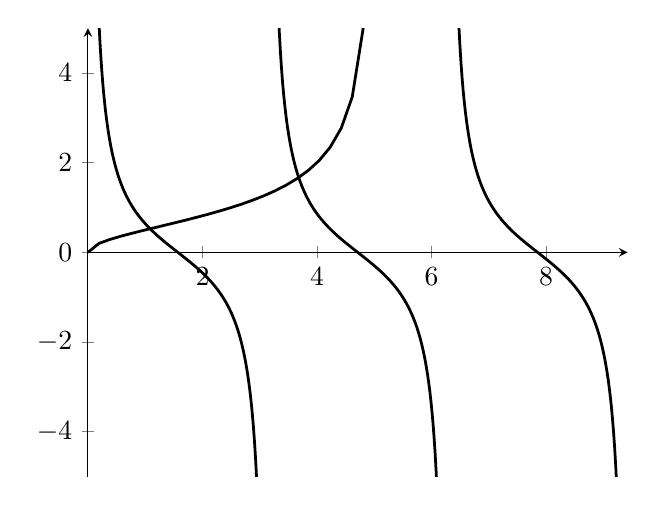
\begin{tikzpicture}cap=round,>=latex]
	\begin{axis}[grid=none,
	axis x line=middle,
	axis y line=left,	
	%enlargelimits,
	%xtick={-1,0,1},
	%xticklabels={$-a$, $0$, $a$},
	%ytick={1},
	%yticklabels={$U_0$},
	%domain=0:700
	xmin=0,
	xmax=3*pi,
	ymin=-5,
	ymax=5,
	restrict y to domain=-10:10 
	]
	
	\addplot[no markers, line width=1, samples=50, domain=0:3*pi] {sqrt(x/( 5-x))};
	\addplot[no markers, line width=1, samples=500, domain=0:3*pi] {cot(deg(x))};	
	\end{axis}								
\end{tikzpicture}
					\caption{Graphical solution to \ref{symtranceq}}
				\end{figure}
				
				In the limit case of $U_0 \rightarrow \infty$,
				\begin{align}
					\frac{k}{\kappa} =& \cot(\frac{kd}{2}),\qquad \kappa \rightarrow \infty \Rightarrow \\
					\cot(\frac{kd}{2}) =& 0 \Rightarrow\qquad	\cos(\frac{kd}{2}) = 0 \Rightarrow\\
					\frac{kd}{2} =& \frac{\pi}{2} + \pi n \\
					k_n =& \frac{\Pi + 2\pi n}{d} \\
					E_n =& \frac{\hbar^2}{2m}\frac{1}{d^2}\left(\pi + 2\pi n\right)^2
				\end{align}
				Which corresponds to the symmetric solutions found earlier to the infinite quantum well problem.
				
			\paragraph{Antisymmetric solutions}
				
				\begin{align}
					Be^{-\kappa \frac{d}{2}} &= D' \sin(\frac{kd}{2}) \\
					\kappa Be^{-\kappa \frac{d}{2}} &= -kD' \cos(\frac{kd}{2})			
				\end{align}
				Or in matrix form:
				\begin{equation}
				\begin{pmatrix}
				e^{-\kappa \frac{d}{2}}			&	-\sin{\frac{kd}{2}}	\\ 
				\kappa e^{-\kappa \frac{d}{2}}	&	k\cos{\frac{kd}{2}}	\\
				\end{pmatrix}
				\begin{pmatrix}
				B \\
				D' \\
				\end{pmatrix}
				=
				\begin{pmatrix}
				0 \\
				0 \\
				\end{pmatrix}			
				\end{equation}
				This system has non-trivial solutions when the determinant of the matrix is equal to zero:
				\begin{align}
					\begin{vmatrix}
						e^{-\kappa \frac{d}{2}}			&	-\sin{\frac{kd}{2}}	\\ 
						\kappa e^{-\kappa \frac{d}{2}}	&	k\cos{\frac{kd}{2}}	\\
					\end{vmatrix}
					=& e^{-\kappa\frac{d}{2}} k\cos{\frac{kd}{2}} + \kappa e^{-\kappa \frac{d}{2}} \sin{\frac{kd}{2}} =\\
					=& k\cos(\frac{kd}{2}) + \kappa\sin(\frac{kd}{2}) = 0 \\
					\frac{k}{\kappa} =& -\tan(\frac{kd}{2}) \label{antisymtranceq}
				\end{align}
				
				With solutions to \ref{antisymtranceq} defining the number of bound states in the quantum well. 
				
				\hl{Knowing to expressions for $k$ and $\kappa$, equation \ref{antisymtranceq} can we written as:}
				\begin{equation}
				\sqrt{\frac{E}{U_0-E}} = -\tan\left(\sqrt{\frac{2m(E+U_0)}{\hbar^2}\frac{d}{2}}\right)
				\end{equation}
				Which can be easily plotted, giving us graphical solutions to Equation \ref{antisymtranceq}.
				\begin{figure}[!h]
					\centering
					\input{figs/analytic/antisymsoleq.tex}
					\caption{Graphical solution to \ref{antisymtranceq}}
				\end{figure}
				
				In the limit case of $U_0 \rightarrow \infty$,
				\begin{align}
					\frac{k}{\kappa} =& -\tan(\frac{kd}{2}),\qquad \kappa \rightarrow \infty \Rightarrow \\
					\tan(\frac{kd}{2}) =& 0 \Rightarrow\qquad	\sin(\frac{kd}{2}) = 0 \Rightarrow\\
					\frac{kd}{2} =& \pi n \\
					k_n =& \frac{2\pi n}{d} \\
					E_n =& \frac{\hbar^2}{2m}\frac{1}{d^2}\left(2\pi n\right)^2
				\end{align}
				Which corresponds to antisymmetric solutions found earlier to the infinite quantum well problem.		
				
			\begin{figure}[!h]
				\centering
				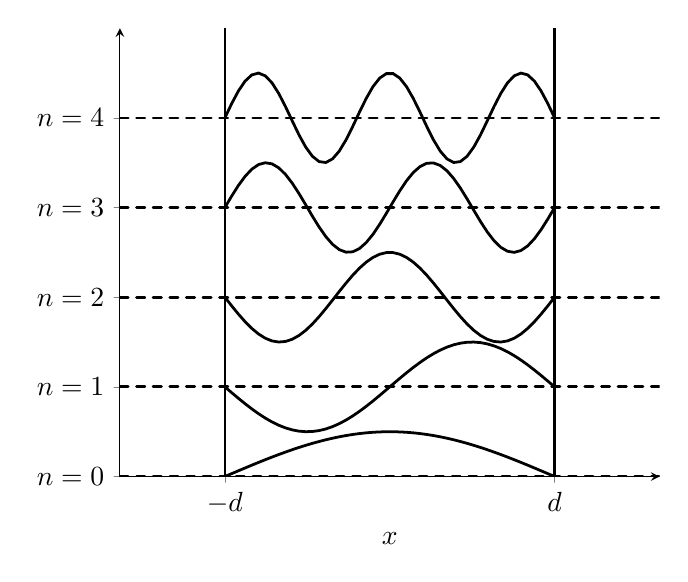
\begin{tikzpicture}[cap=round,>=latex]
\begin{axis}[grid=none,
axis x line=bottom,
axis y line=left,	
%enlargelimits,
xtick={0,3.1415},
xticklabels={$-d$, $d$},
ytick={0,2,4,6,8},
yticklabels={$n = 0$,$n = 1$, $n = 2$, $n = 3$, $n = 4$},
xlabel={$x$},
xmin=-1,
xmax=pi+1,
ymin=0,
ymax=10,
]

%sym 0
\addplot[no markers, line width=1, samples=50, domain=0:pi] {cos(deg(x-pi/2))};

%\addplot[no markers, line width=1, samples=50, domain=-1:0.3]{exp(x)*(cos(deg(0.3-pi/2)))+0.5};
%\addplot[no markers, line width=1, samples=50, domain=pi-0.3:pi+1]{exp(-x+pi-0.3)*(cos(deg(pi-0.3))+0.5)};
\addplot[no markers, dashed, line width=1, samples=50, domain=-1:pi+1]{0};

%antisym 1
\addplot[no markers, line width=1, samples=50, domain=0:pi] {sin(deg(2*(x-pi/2)))+2};
\addplot[no markers, dashed, line width=1, samples=50, domain=-1:pi+1]{2};

%sym 2
\addplot[no markers, line width=1, samples=50, domain=0:pi] {cos(deg(3*(x-pi/2)))+4};
\addplot[no markers, dashed, line width=1, samples=50, domain=-1:pi+1]{4};

%antisym 3
\addplot[no markers, line width=1, samples=50, domain=0:pi] {sin(deg(4*(x-pi/2)))+6};
\addplot[no markers, dashed, line width=1, samples=50, domain=-1:pi+1]{6};

%sym 2
\addplot[no markers, line width=1, samples=50, domain=0:pi] {cos(deg(5*(x-pi/2)))+8};
\addplot[no markers, dashed, line width=1, samples=50, domain=-1:pi+1]{8};

\addplot [no markers, line width=1] coordinates {(0, 0) (0, 10)};
\addplot [no markers, line width=1] coordinates {(pi, 0) (pi, 10)};
\end{axis}								


\end{tikzpicture}

				\caption{\hl{Quantum well bound state wave functions}}
			\end{figure}
			For $E > U_0$, the states of the system form a continuous spectrum of waves propagating in either direction.
		\subsubsection{Propagating states in a system of potential barriers}
			\begin{figure}[!h]
				\centering
				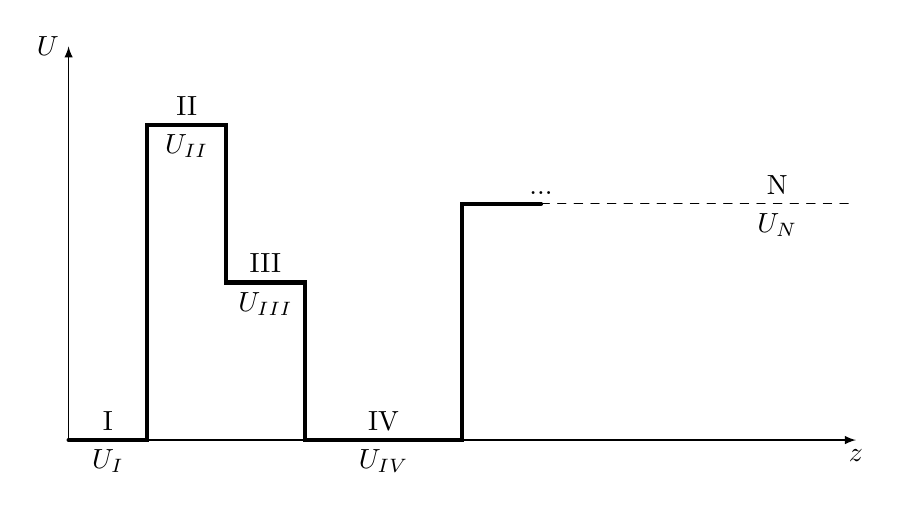
\begin{tikzpicture}[scale=1,cap=round,>=latex]
	\draw [<->] (-5, 5) -- (-5, 0) -- (5, 0);
	\node [left] at (-5, 5) {$U$};
	\node [below] at (5, 0) {$z$};
	
	\draw [line width=1.5] (-5, 0) -- (-4, 0) -- 
							(-4, 4) -- (-3, 4) -- 
							(-3, 2) -- (-2, 2) --
							(-2, 0) -- (0, 0) --
							(0, 3) -- (1, 3);
	\draw [dashed] (1, 3) -- (5, 3);
	
	\node [above] at (-4.5, 0) {I};
	\node [below] at (-4.5, 0) {$U_I$};

	\node [above] at (-3.5, 4) {II};
	\node [below] at (-3.5, 4) {$U_{II}$};
	
	\node [above] at (-2.5, 2) {III};
	\node [below] at (-2.5, 2) {$U_{III}$};

	\node [above] at (-1, 0) {IV};
	\node [below] at (-1, 0) {$U_{IV}$};
	
	\node [above] at (1, 3) {...};
		
	\node [above] at (4, 3) {N};
	\node [below] at (4, 3) {$U_{N}$};


	%\node [below] at (-1, 0) {$-\frac{d}{2}$};
	%\node [below] at (0, 0) {$\frac{d}{2}$};
	
\end{tikzpicture}
				\caption{System of potential barriers}
			\end{figure}			
			The system and be separated into two cases: propagation through a region, and reflection/transmission through a barrier, these cases correspond to solutions of the Shr\"odinger equation in each of the regions and to the boundary conditions between the regions.
			
			The wavefunction at each point of the system can be written as a sum of forward and backward propagating waves:
			\begin{align}
				\Psi|_{z=z_{0}} =& Ae^{ikz_0} + Be^{-ikz_0} \\
				\Psi|_{z=z_{0}+d} =& Ae^{ikz_0}e^{ikd} + Be^{-ikz_0}e^{-ikd}				
			\end{align}
			or, in vector form:
			\begin{equation}
				\Psi = 
				\begin{pmatrix}
				A_+ \\
				A_- \\
				\end{pmatrix}
			\end{equation}
			
			In that case, equations \hl{REF} can be rewritten as a matrix equation:
			\begin{align}
				\Psi|_{z=z_{0}} =& 
				\begin{pmatrix}
					A_+ \\
					A_- \\
				\end{pmatrix} \\
				\Psi|_{z=z_{0}+d} =&
				\begin{pmatrix}
					A_+' \\
					A_-' \\
				\end{pmatrix}				
				= \begin{pmatrix}
					A_+ \\
					A_- \\
				\end{pmatrix} \hat{M} = \Psi|_{z=z_{0}} \hat{M}
			\end{align}
			
			If both $z_0$ and $z_0 + d$ correspond to the same region of the system of barriers, then matrix $\hat{M}$ is simply a propagation matrix:
			\begin{equation}
				\hat{P} = \begin{pmatrix}
				e^{ikd} & 0 \\
				0		& e^{-ikd}
				\end{pmatrix}
			\end{equation}
			
			To build a matrix corresponding to the boundary between regions, he have to start with a different basis, in which we can easily write the boundary conditions:
			
			\begin{align}
				\begin{pmatrix}	
					\Psi_{I} \\
					\frac{\partial \Psi_{I}}{\partial z}
				\end{pmatrix} =& 
				\hat{I} \begin{pmatrix}	
					\Psi_{II} \\
					\frac{\partial \Psi_{II}}{\partial z}
				\end{pmatrix} \\
				\hat{I} =& \begin{pmatrix}
					\hl{explicit} & \hl{explicit} \\
					\hl{explicit} & \hl{explicit} 					
					\end{pmatrix}
			\end{align}
			
			The basis	$\left(\begin{smallmatrix}	
				\Psi_{I} \\
				\frac{\partial \Psi_{I}}{\partial z}
			\end{smallmatrix}\right)$ can be easily written in terms of the basis $\left(\begin{smallmatrix}
				A_+' \\
				A_-' \\
			\end{smallmatrix}\right)$:
			
			\begin{align}
				\Psi =& A_+ e^{ikz} + A_- e^{-ikz} \\
				\frac{\partial \Psi}{\partial z} =& ikA_+ e^{ikz} - ikA_- e^{-ikz} \\
				\begin{pmatrix}	
					\Psi \\
					\frac{\partial \Psi}{\partial z}
				\end{pmatrix} =& 
				\begin{pmatrix}
					1 & 1 \\
					ik & -ik \\
				\end{pmatrix}
				\begin{pmatrix}
					A_+ \\
					A_- \\
				\end{pmatrix} = \hat{S} 
				\begin{pmatrix}
					A_+ \\
					A_- \\
				\end{pmatrix}
			\end{align}
			
			Meaning that 
			\begin{align}
				\begin{pmatrix}	
					\Psi \\
					\frac{\partial \Psi}{\partial z}
				\end{pmatrix}
				= \hat{S} 
				\begin{pmatrix}
					A_+ \\
					A_- \\
				\end{pmatrix} \qquad\&&\qquad
				\begin{pmatrix}
					A_+ \\
					A_- \\
				\end{pmatrix} = \hat{S}^-1
				\begin{pmatrix}	
					\Psi \\
					\frac{\partial \Psi}{\partial z}
				\end{pmatrix} \\
				\begin{pmatrix}	
					\Psi_{I} \\
					\frac{\partial \Psi_{I}}{\partial z}
				\end{pmatrix} =& 
				\hat{I} \begin{pmatrix}	
					\Psi_{II} \\
					\frac{\partial \Psi_{II}}{\partial z}
					\end{pmatrix} \\
				\hat{S} 
				\begin{pmatrix}
					A_{I+} \\
					A_{I-} \\
				\end{pmatrix} =& 
				\hat{I}\hat{S} 
				\begin{pmatrix}
					A_{II+} \\
					A_{II-} \\
				\end{pmatrix} \\
				\begin{pmatrix}
					A_{I+} \\
					A_{I-} \\
				\end{pmatrix} =& 
				\hat{S}^{-1}\hat{I}\hat{S} 
				\begin{pmatrix}
					A_{II+} \\
					A_{II-} \\
				\end{pmatrix} \\
				\begin{pmatrix}
					A_{I+} \\
					A_{I-} \\
				\end{pmatrix} =& 
				\hat{M} 
				\begin{pmatrix}
					A_{II+} \\
					A_{II-} \\
				\end{pmatrix},\qquad \hat{M} = \hat{S}^{-1}\hat{I}\hat{S} \\
				\hl{\det{\hat{M}}} =& 1
			\end{align}
			Meaning that we can represent a whole series of potential wells and barriers as a product of their \textit{transfer} matricies:
			\begin{equation}
				\Psi_n = \hat{T_n}\hat{T_{n-1}}...\hat{T_2}\hat{T_1}\Psi_0, \qquad \hat{T_i} = \hat{M}_{i-1\rightarrow i}\hat{P_i} 
			\end{equation}
			
			Transfer matricies can also be used to find the bound states or eigenmodes of the system:
			\hl{Wait, what?}
			\begin{align}
				\hat{\Psi}_{\frac{d}{2}} =& \hat{\Psi}_{-\frac{d}{2}} \\
				\begin{pmatrix}
					Ae^{-\kappa \frac{d}{2}} \\
					-\kappa Ae^{-\kappa \frac{d}{2}} \\
				\end{pmatrix} =& \hat{T} 
				\begin{pmatrix}
					Be^{-\kappa \frac{d}{2}} \\
					\kappa Ae^{-\kappa \frac{d}{2}} \\
				\end{pmatrix}
			\end{align}
			
			Using transfer matricies, the calculation of an electron's probability of tunneling through a barrier is equivalent to solving the following matrix equation:
			\begin{align}
				\begin{pmatrix}
					t \\
					0
				\end{pmatrix} = \hat{M}
				\begin{pmatrix}
					1 \\
					r
				\end{pmatrix} \\
				r  = -\frac{M_{21}}{M_{22}} \\
				t = \frac{1}{M_{22}}
			\end{align}
	\subsection{Harmonic oscillator}
	\label{sec:harmonic}

	Using the classical harmonic oscillator equation, we can write the Hamiltonian for a quantum harmonic equation:
	\begin{align}
		m\ddot{x} = -kx \\
		E = E_{kin} + U = \frac{mv^2}{2} + \frac{mx^2}{2} = \frac{p^2}{2m} + \frac{kx^2}{2} \\
		\hat{H} = \frac{\hat{p}^2}{2m} + \frac{m\omega^2\hat{x}^2}{2}, \quad \omega = \sqrt{\frac{k}{m}}
	\end{align}
	
	The Schr\"odinger equation:
	\begin{align}
		\hat{H}\Psi = E\Psi, \quad \hat{p} = -i\hbar\frac{\partial}{\partial x} \\
		\left[\frac{-i\hbar^2}{2m} \frac{\partial^2}{\partial x^2} + \frac{m\omega^2x^2}{2}\right]\Psi(x) = E\Psi(x) \\
		\Psi|_{x = \pm \infty} = 0
	\end{align}
	
	Lets define two new operators, $\hat{a}^+$ and $\hat{a}$ and their composition $\hat{N} = \hat{a}^+\hat{a}$:
	\begin{align}
		\hat{a}^+ =& \sqrt{\frac{m\omega}{2\hbar}}\left(\hat{x} + \frac{i\hat{p}}{2m}\right) \\
		\hat{a} =& \sqrt{\frac{m\omega}{2\hbar}}\left(\hat{x} - \frac{i\hat{p}}{2m}\right) \\
		\hat{N} = \hat{a}^+\hat{a} =& \frac{m\omega}{2\hbar}\left(\hat{x} + \frac{i\hat{p}}{2m}\right)\left(\hat{x} - \frac{i\hat{p}}{2m}\right)\\
		=& \frac{m\omega}{2\hbar}\left( x^2 - \frac{i\hat{p}\hat{x}}{m\omega} + \frac{i\hat{x}\hat{p}}{m\omega} + \frac{\hat{p}^2}{m^2\omega^2} \right)\\
		=& \frac{m\omega}{2\hbar}\left(x^2 + \frac{\hat{p}^2}{m\omega} + \frac{i}{m\omega}\left[\hat{x}, \hat{p}\right]\right)\\
		=&\frac{m\omega}{2\hbar}\left(x^2 + \frac{\hat{p}^2}{m\omega} - \frac{\hbar}{m\omega}\right)\\
		=& \frac{m\omega x^2}{2\hbar} + \frac{\hat{p}^2}{2\hbar m\omega} - \frac{1}{2}\\
		=& \frac{\hat{H}}{\hbar\omega} - \frac{1}{2}\\
		\hat{H} =& \hbar\omega\left(\hat{N} + \frac{1}{2}\right)\quad \left[\hat{H}, \hat{N}\right] = 0
	\end{align}

	\begin{align}
		\left. N | n \right\rangle =& \left. n |n \right\rangle \\
		\left. \hat{H} | n \right\rangle =& \left. \hbar\omega\left(\hat{N} + \frac{1}{2}\right) | n \right\rangle\\
		 =& \left. \hbar\omega\left(n + \frac{1}{2}\right) | n \right\rangle = \left. E_n | n \right\rangle\\		
	\end{align}

	\begin{align}
		\left[\hat{a}^+, \hat{a}\right] =& \frac{m\omega}{2\hbar}\left[\hat{x} + \frac{i\hat{p}}{2m}, \hat{x} - \frac{i\hat{p}}{2m}\right]\\
		=& \frac{m\omega}{2\hbar}\left[(\hat{x}^2 - \frac{i\hat{p}\hat{x}}{2m} + \frac{i\hat{x}\hat{p}}{2m} +\frac{\hat{p}^2}{4m^2}) - (\hat{x}^2  - \frac{i\hat{x}\hat{p}}{2m} + \frac{i\hat{p}\hat{x}}{2m} +\frac{\hat{p}^2}{4m^2})\right] \\
		=& \frac{m\omega}{2\hbar}\left[\frac{i\hat{x}\hat{p}}{m} -\frac{i\hat{p}\hat{x}}{m}\right]\\
		=& \frac{i}{\hbar}\left[\hat{x}, \hat{p}\right] = -1 \text{\hl{???}}
	\end{align}

	\begin{align}
		\left[\hat{N}, \hat{a}\right] =& \left[\hat{a}^+\hat{a}, \hat{a}\right]\\
		 =& \hat{a}^+\left[\hat{a}, \hat{a}\right]+\left[\hat{a}^+, \hat{a}\right]\hat{a} = -\hat{a}
	\end{align}
	
	\begin{align}
		\left. \hat{N} | n \right\rangle =& \left. n | n \right\rangle \\
		\left. \hat{N}\hat{a}^+ | n \right\rangle =& \left. \left(\left[\hat{N}, \hat{a}^+\right] + \hat{a}^+\hat{N}\right)|n\right\rangle\\ 
		=& \left. \left(\hat{a}^+ + \hat{a}^+\hat{N}\right)|n\right\rangle\\ 
		=& \left.\left(n+1\right)\hat{a}^+|n\right\rangle \\
		\left. \hat{N}\hat{a} | n \right\rangle =& \left. \left(\left[\hat{N}, \hat{a}\right] + \hat{a}\hat{N}\right)|n\right\rangle\\ 
		=& \left. \left(-\hat{a} + \hat{a}\hat{N}\right)|n\right\rangle\\ 
		=& \left.\left(n-1\right)\hat{a}|n\right\rangle		
	\end{align}

	Know this we can write:
	\begin{align}
		\left. \hat{a}|n\right\rangle =& \left. c | n-1 \right\rangle \\
		\left. \hat{a}^+|n\right\rangle =& \left. c' | n+1 \right\rangle \\		
	\end{align}

	\begin{align}
		\left\langle n | \hat{a}^+\hat{a} | n \right\rangle =& n = |c|^2 \geq 0 \\
		\left\langle n - 1 | n - 1 \right\rangle =& 1 \\
		\left\langle n - 1 | \hat{a}^+\hat{a} | n - 1 \right\rangle =& |c|^2 \\	
		\left. \hat{a} | n \right\rangle =& \left.\sqrt{n}|n-1\right\rangle \\
		\left. \hat{a}^+| n \right\rangle =& \left.\sqrt{n+1}|n+1\right\rangle \\		
	\end{align}


	\begin{align}
		\left. \hat{a} | n \right\rangle =& \left.\sqrt{n}|n-1\right\rangle \\
		\left. \hat{a}^2 | n \right\rangle =& \left.\sqrt{n}\sqrt{n-1}|n-2\right\rangle \\
		\left. \hat{a} | 2,3 \right\rangle =& \left.\sqrt{2,3}|1,3\right\rangle \\
		\left. \hat{a}^2 | 2,3 \right\rangle =& \left.\sqrt{2,3}\sqrt{1,3}|0,3\right\rangle \\		
		\left. \hat{a}^3 | 2,3 \right\rangle =& \left.\sqrt{2,3}\sqrt{1,3}\sqrt{0,3}|-0,7\right\rangle \\		
		\left. \hat{a}^4 | 2,3 \right\rangle =& \left.\sqrt{2,3}\sqrt{1,3}\sqrt{0,3}\sqrt{-0,7}|-1,7\right\rangle \Rightarrow\\				
		\left. \hat{a}^n | n \right\rangle =& \sqrt{0}, \quad n  \in \mathds{N}
	\end{align}


	\subsection{Angular momentum}
	\label{sec:angmomentum}
	\subsubsection{Classical}
	\begin{figure}[!h]
		\centering
		\tdplotsetmaincoords{80}{60}

\begin{tikzpicture}[scale=5,tdplot_main_coords]
\coordinate (O) at (0,0,0);
\draw[thick,->] (0,0,0) -- (1,0,0) node[anchor=north east]{$\vec{r}$};
\draw[thick,->] (1,0,0) -- (1,0,1) node[anchor=south]{$\vec{p}$};
\draw[thick,->] (0,0,0) -- (0,2,0) node[anchor=north west]{$\vec{L}$};

\tdplotsetthetaplanecoords{0}
\draw[dashed,tdplot_rotated_coords] (1,0,0) arc (0:360:1);

\end{tikzpicture}
		\caption{Classical angular momentum}
		\label{clasmoment}
	\end{figure}
	
	\begin{align}
		\vec{L} =& \vec{r}\times\vec{p} =
		\begin{vmatrix}
			\vec{e_x} & \vec{e_y} & \vec{e_z} \\
			x & y & z \\
			p_x & p_y & p_z \\
		\end{vmatrix} \\
		=& \vec{e_x}(yp_z - zp_y) + \vec{e_y}(zp_x - xp_z) + \vec{e_z}(xp_y - yp_x) \\
		=& \vec{e_x}L_x + \vec{e_y}L_y + \vec{e_z}L_z
	\end{align}
	
	%Building on classical angular momentum is the Rutherford atomic model:
	%\begin{figure}[!h]
	%	\centering
	%	
\begin{tikzpicture}[scale=2,cap=round,>=latex]
	\draw [line width=2] (-2, -2) -- (-2, 2) -- (2, 2) -- (2, -2) -- (-2, -2);
	
	\node at (0, 0) {placeholder};
\end{tikzpicture}
	%	\caption{Rutherford atom}
	%	\label{ruthatom}
	%\end{figure}
	%
	%\begin{align}
	%	\frac{mv^2}{r} =& \frac{ke^2}{r^2} \\
	%	m\vec{a} =& \vec{F_c}
	%\end{align}
	%
	%\begin{list}[Problems with the Rutherford model]
	%	\item Discrete energy levels
	%	\item 
	%\end{list}
	\subsubsection{Quantum}
	\begin{align}
		\hat{\vec{p}} =& -i\hbar\vec{\nabla}, \qquad \vec{\nabla} = \vec{e_x}\frac{\partial}{\partial x} + \vec{e_y}\frac{\partial}{\partial y} + \vec{e_z}\frac{\partial}{\partial z} \\
		p_x =& -i\hbar \frac{\partial}{\partial x}, \quad p_y = -i\hbar \frac{\partial}{\partial y}, \quad p_z = -i\hbar \frac{\partial}{\partial z} \\
		\hat{\vec{L}} =& -i\hbar\vec{r}\times\vec{\nabla} \\
		\hat{L_x} =& -i\hbar(y\frac{\partial}{\partial z} - z\frac{\partial}{\partial y}), \quad \hat{L_y} = -i\hbar(z\frac{\partial}{\partial x} - x\frac{\partial}{\partial z}), \quad \hat{L_z} = -i\hbar(y\frac{\partial}{\partial x} - x\frac{\partial}{\partial y}) 
	\end{align}
	
	\hl{Proof!} Commutators:
	\begin{equation}
	\left[\hat{L_x}, \hat{L_y}\right] = i\hbar\hat{L_z}, \quad
	\left[\hat{L_z}, \hat{L_x}\right] = i\hbar\hat{L_y}, \quad
	\left[\hat{L_y}, \hat{L_z}\right] = i\hbar\hat{L_x}
	\end{equation}
	
	Uncertainty: \hl{Wait, what?}
	\begin{align}
		\Delta \hat{L_x} = \hat{L_x} - \left<\hat{L_x} \right>, \quad
		\Delta \hat{L_y} = \hat{L_y} - \left<\hat{L_y} \right>, \quad
		\Delta \hat{L_z} = \hat{L_z} - \left<\hat{L_z} \right> \\
		\left<(\Delta\hat{L_x})^2 \right> = \left<\hat{L_x}^2 \right> - \left<\hat{L_x} \right>^2 \\
		\left<(\Delta\hat{L_y})^2 \right> = \left<\hat{L_y}^2 \right> - \left<\hat{L_y} \right>^2 \\
		\left<\hat{L_x} \right> = \int \Psi^* \hat{L_x} \Psi dV \\ 
		\left<(\Delta\hat{L_x})^2 \right>\left<(\Delta\hat{L_y})^2 \right> \geq \frac{\hbar^2|\left<\hat{L_z}\right>|^2}{4} \\
		\left<(\Delta x)^2 \right>\left<(\Delta p_x)^2 \right> \geq \frac{\hbar^2}{4} \nonumber				
	\end{align}
	
	Generally it isn't possible to measure $L_x, L_y, L_z$ at once. 
	
	Total momentum:
	\begin{align}
		\hat{L}^2 =& \hat{L_x}^2 + \hat{L_y}^2 + \hat{L_z}^2 \\
		\left[\hat{L}^2, \hat{L_x}^2\right] =& \left[\hat{L}^2, \hat{L_y}^2\right] = \left[\hat{L}^2, \hat{L_z}^2\right] = 0 \\
		|\vec{L}| =& \sqrt{\hat{L_x}^2 + \hat{L_y}^2 + \hat{L_z}^2}								
	\end{align}
	
	\paragraph{Hydrogen atom}		
	Using the definitions of $\hat{L_x}$ and $\hat{L}^2$ we can begin to solve the hydrogen atom:
	
	\begin{align}
		\left\{ \begin{aligned}
			\hat{L}^2 \Psi =& L^2 \Psi \\
			\hat{L_z} \Psi =& L_z \Psi  
		\end{aligned} \right. \\
		\Psi~-? \quad L~-&? \quad L_z~-? \nonumber
		\label{hydrogensystem1}
	\end{align}
	
	This system of equations is easy to solve in spherical coordinates:
	\begin{figure}[!h]
		\centering
		\tdplotsetmaincoords{60}{110}

\begin{tikzpicture}[scale=5,tdplot_main_coords]
	\pgfmathsetmacro{\rvec}{.8}
	\pgfmathsetmacro{\thetavec}{30}
	\pgfmathsetmacro{\phivec}{60}

    \coordinate (O) at (0,0,0);
    \draw[thick,->] (0,0,0) -- (1,0,0) node[anchor=north east]{$x$};
    \draw[thick,->] (0,0,0) -- (0,1,0) node[anchor=north west]{$y$};
	\draw[thick,->] (0,0,0) -- (0,0,1) node[anchor=south]{$z$};
    \tdplotsetcoord{P}{\rvec}{\thetavec}{\phivec}
    \draw[-stealth,color=red] (O) -- (P) node[above right] {$r$};
    \draw[dashed, color=red] (O) -- (Pxy);
    \draw[dashed, color=red] (P) -- (Pxy);
    \tdplotdrawarc{(O)}{0.2}{0}{\phivec}{anchor=north}{$\phi$}
    \tdplotsetthetaplanecoords{\phivec}
    \tdplotdrawarc[tdplot_rotated_coords]{(0,0,0)}{0.5}{0}%
        {\thetavec}{anchor=south west}{$\theta$}


\end{tikzpicture}
		\caption{Spherical coordinates}
	\end{figure}
	
	\begin{align}
		z =& r \cos(\theta) \\ 
		x =& r \cos(\theta)\sin(\phi) \\ 
		y =& r \cos(\theta)\cos(\phi) \\ 								
	\end{align}
	
	\begin{align}
		\left\{ \begin{aligned}
			\hat{L_x} =& - i\hbar \left(\sin(\phi)\frac{\partial}{\partial \theta} + \cot(\theta)\cos(\phi)\frac{\partial}{\partial \phi}\right) \\
			\hat{L_y} =& - i\hbar \left(\cos(\phi)\frac{\partial}{\partial \theta} - \cot(\theta)\sin(\phi)\frac{\partial}{\partial \phi}\right) \\
			\hat{L_z} =& - i\hbar \frac{\partial}{\partial \phi}
		\end{aligned} \right.
	\end{align}
	
	\hl{Check}
	\begin{align}
		\hat{L}^2 	&= \hat{L_x}^2 + \hat{L_y}^2 + \hat{L_z}^2 = \\
		&= -\hbar^2 \left( \frac{\partial^2}{\partial \phi^2} + \left(\sin^2(\theta) + \cos^2(\theta) \right)\frac{\partial^2}{\partial \theta^2} + \cot^2(\theta) \frac{\partial^2}{\partial \phi^2} \right) = \\
		&= -\hbar^2 \Delta_{\theta, \phi} \\
		\Delta_{\theta, \phi} &= \frac{1}{\sin (\theta)}\frac{\partial}{\partial \theta}\left(\sin(\theta)\frac{\partial}{\partial \theta}\right) + \frac{1}{\sin^2(\theta)}\frac{\partial^2}{\partial \phi ^2}
	\end{align}
	
	Which allows us to rewrite \ref{hydrogensystem1} as:
	
	\begin{align}
		\left\{ \begin{aligned}
			-\hbar^2 \Delta_{\theta, \phi} \Psi = L^2 \Psi \\
			-i\hbar \frac{\partial \Psi}{\partial \phi} = L_z \Psi
		\end{aligned} \right.				
	\end{align}
	
	Since $\theta$ and $\phi$ are independent variables, we can first solve the equation for $L_z(\phi)$, and then use that solution to solve for $L(\theta, \phi)$. The whole hydrogen atom system is defined as follows (disregarding spin):
	
	\begin{align}
		\left\{ \begin{aligned}
			\hat{H} \Psi =& E \Psi \rightarrow n\\
			\hat{L}^2 \Psi =& L^2 \Psi \rightarrow l \\
			\hat{L_z} \Psi =& L_z \Psi  \rightarrow m
		\end{aligned} \right. \\
		\Rightarrow \Psi_{n,l,m}
	\end{align}
	\subsection{Spherically symmetric potential}
		The Hamiltonian for a particle in a center-symmetric potential is written as:
		\begin{equation}
			\hat{H} = \frac{\hbar^2}{2m}\Delta + U(r)
		\end{equation}
		Where $\Delta$ in spherical coordinates is
		\begin{equation}
			\Delta = \frac{1}{r}\frac{\partial^2}{\partial r ^2}r + \frac{1}{r^2} \frac{\partial^2}{\partial \theta^2} + \frac{1}{\tan(\theta)}\frac{\partial}{\partial \theta} + \frac{1}{\sin(\theta)}\frac{\partial^2}{\partial \phi^2}
		\end{equation}
		\hl{Which is very similar to $\hat{\vec{L}}$}.
		\begin{align}
			\hat{\vec{L}} =& \vec{r}\times\hat{\vec{p}} = -i\hbar\vec{r}\times\nabla \\
			\hat{H} =& \hat{R}(|r|) + \frac{1}{2m r^2}\hat{\vec{L}}
		\end{align}
		Since \hl{$\left[\hat{H}, \hat{\vec{L}}\right] = 0$},
		\begin{equation}
			i\hbar\frac{d\hat{\vec{L}}}{dt} = \left[\hat{H}, \hat{\vec{L}}\right] = 0
		\end{equation}
		Meaning that $\hat{\vec{L}}$ is a conserved value \hl{eigenvalue}.
		
		\hl{????}
		\begin{align}
			i\hbar\frac{d\hat{\vec{p}}}{dt} =& \left[\hat{H}, \hat{\vec{p}}\right] \\
			\frac{d\hat{\vec{p}}}{dt} =& -DU = -\frac{\partial U(r)}{\partial t}
		\end{align}
		
		Using defintions from Section \ref{sec:angmomentum}, we have
		\begin{align}
			\hat{\vec{L}} = \left(\hat{L_x}, \hat{L_y}, \hat{L_z}\right) \\
			\left[\hat{H}, \hat{L_i}\right] = 0, \qquad \left[\hat{H}, \hat{L}^2\right] = 0 \\
			\left\{ \begin{aligned}
				\left[\hat{L_x}, \hat{L_y}\right] = i\hbar\hat{L_z} \\
				\left[\hat{L_y}, \hat{L_z}\right] = i\hbar\hat{L_x} \\
				\left[\hat{L_z}, \hat{L_x}\right] = i\hbar\hat{L_y}
			\end{aligned} \right. \\			
			\left[\hat{L}^2, \hat{L_z}\right] = 0
		\end{align}
		It is convenient to introduce two new operators, similar to $\hat{a_+}, \hat{a_-}$ from Sec.\ref{sec:harmonic}:
		\begin{align}
			\hat{L_+} =& \hat{L_x} + i\hat{L_y} \\
			\hat{L_-} =& \hat{L_x} - i\hat{L_y}	\\
			\left[\hat{L_+}, \hat{L_-}\right] =& \left[\hat{L_x}, \hat{L_x}\right] + i\left[\hat{L_y}, \hat{L_x}\right] \\
			-& i\left[\hat{L_x}, \hat{L_y}\right] + \left[\hat{L_y}, \hat{L_y}\right] \\
			=& -2i\left[\hat{L_x}, \hat{L_y}\right] = 2\hbar\hat{L_z} \\
			\left[\hat{L_z}, \hat{L_-}\right] =& \left[\hat{L_z}, \hat{L_x} -i\hat{L_y}\right]\\
			=& \left[\hat{L_z}, \hat{L_x}\right] - i\left[\hat{L_z}, \hat{L_y}\right]\\
			=& i\hbar\hat{L_y} -\hbar\hat{L_x} = -\hbar\hat{L_-} \\
			\left[\hat{L_z}, \hat{L_+}\right] =& -\hbar\hbar{L_+}
		\end{align}
		
		\begin{align}
			\hat{L_+}\hat{L_-} =& \hat{L_x}^2 + \hat{L_y}^2 + i\left(\hat{L_y}\hat{L_x} - \hat{L_x}\hat{L_y}\right) \\
			=& \hat{L_x}^2 + \hat{L_y}^2 + \hbar\hat{L_z} \\
			=& \hat{\vec{L}}^2 - \hat{L_z}^2 + \hbar\hat{L_z}
		\end{align}
		
		Using these definitions, we can calculate the eigenvalues of $\hat{\vec{L}}^2$ and $\hat{L_z}$.
		
		\begin{align}
			\hat{\vec{L}}^2 =& \frac{1}{2}\left(\hat{L_+}\hat{L_-} - \hat{L_-}\hat{L_+}\right) + \hat{L_z}^2 \\
			\hat\vec{{L}}^2 =& \hat{L_x}^2 + \hat{L_y}^2 + \hat{L_z}^2
		\end{align}
		Which means that $\hat{\vec{L}}^2$ is positive, meaning that its eigenvalues are not negative:
		\begin{align}
			\left\langle \Psi | \hat{\vec{L}} | \Psi \right\rangle \geq& 0 \\
			\lambda\left\langle \Psi | \Psi \right\rangle \geq& 0 \\
			\lambda \geq& 0 
		\end{align}
		
		A positive and real number can be represented as $j(j + 1)$, meaning that:
		\begin{align}
			\lambda =& \hbar^2 j(j+1) \\
			\left. \hat{\vec{L}}^2 | \Psi \right\rangle =& \left. \hbar^2 j(j+1)| \Psi \right\rangle \\
			\left. \hat{L_z} | \Psi \right\rangle =& \left. \hbar m | \Psi \right\rangle \\
			\left. |\Psi \right\rangle =& \left. |j,m \right\rangle \\ 
		\end{align}
		Knowing this, we can write:
		\begin{align}
			\left|\left. \hat{L_+}|j,m\right\rangle\right|^2 =& \left\langle j,m |\hat{L_-}|\hat{L_+}| j,m \right\rangle = \left\langle j,m |\hat{\vec{L}}^2 - \hat{L_z}^2 - \hbar\hat{L_z}| j,m \right\rangle \\
			=& \left(\hbar^2j(j+1) - m^2\hbar^2 - \hbar^2m\right)\left\langle j,m | j,m \right\rangle = \left(\hbar^2j(j+1) - m^2\hbar^2 - \hbar^2m\right) \\
			& \left(\hbar^2j(j+1) - m^2\hbar^2 - \hbar^2m\right) \geq 0 \\
			& (j - m)(j + m) + j-m \geq 0 \\
			& (j - m)(j + m + 1) \geq 0 \Rightarrow\\
			& -j-1 \leq m \leq j
		\end{align}
		\hl{And}:
		\begin{align}
			\left|\left. \hat{L_-}|j,m\right\rangle\right|^2 =& \left\langle j,m |\hat{L_+}|\hat{L_-}| j,m \right\rangle = \hl{...} \\
			& (j + m)(j - m + 1) \geq 0 \Rightarrow\\
			& -j \leq m \leq j + 1
		\end{align}		
		Which means that:
		\begin{equation}
			- j \leq m \leq j		
		\end{equation}
		
		For the two edge cases, $m = j$ and $m = -j$:
		\begin{align}
			m = j& \\
			\left| \left. \hat{L_+} | j,j \right\rangle \right|^2 &= \left\langle j,j | \hat{L_-}| \hat{L_+} |j,j \right\rangle \\
			&= \hbar^2 \left( j(j+1) - j^2 - j\right) = 0 \\
			\left. \hat{L_+} | j,j \right\rangle &= 0 \\
			m = -j& \\
			\left| \left. \hat{L_-} | j,j \right\rangle \right|^2 &= \left\langle j,j | \hat{L_+}| \hat{L_-} |j,j \right\rangle \\
			&= \hbar^2 \left( j(j+1) - (-j)^2 + (-j)\right) = 0 \\
			\left. \hat{L_+} | j,j \right\rangle &= 0 \\			
			\left. \hat{L_-} | j,-j \right\rangle &= 0 \\			
		\end{align}
		Now for $\hat{L_z}$:
		\begin{align}
			\left.\left[L_z, L_-\right]|j,m\right\rangle =& \left.-i\hbar\hat{L_-}|j,m\right\rangle \\
			=& \left.\hat{L_z}\hat{L_-}|j,m\right\rangle - \left.\hat{L_-}\hat{L_z}|j,m\right\rangle = \left.\hat{L_z}\hat{L_-}|j,m\right\rangle - \left.(-i\hbar m)\hat{L_-}|j,m\right\rangle \Rightarrow \\
			\left.\hat{L_z}\hat{L_-}|j,m\right\rangle =& \left. \hbar(m-1)\hat{L_z}|j,m\right\rangle \\
			\left.\left[L_z, L_+\right]|j,m\right\rangle =& \left.i\hbar\hat{L_+}|j,m\right\rangle \\
			=& \left.\hat{L_z}\hat{L_+}|j,m\right\rangle - \left.\hat{L_+}\hat{L_z}|j,m\right\rangle = \left.\hat{L_z}\hat{L_+}|j,m\right\rangle - \left.(-i\hbar m)\hat{L_+}|j,m\right\rangle \Rightarrow \\			
			\left.\hat{L_z}\hat{L_+}|j,m\right\rangle =& \left. \hbar(m+1)\hat{L_z}|j,m\right\rangle \\			
		\end{align}
		Which is very similar to the $\hat{N}\hat{a_+}$ and $\hat{N}\hat{a_-}$ operators from Section \ref{sec:harmonic}.
		
		\begin{align}
			\left.\hat{L_-}|j,m\right\rangle = \left.\alpha|j,m-1\right\rangle \\
			\left.\hat{L_+}|j,m\right\rangle = \left.\alpha|j,m+1\right\rangle \\
		\end{align}
		\paragraph{$\hat{L_-}$}
			If we apply $\hat{L_-}$ $p$ times:
			\begin{align}
				\left. \left(\hat{L_-}\right)^p | j,m \right\rangle &\\
				\left. \hat{L_z}\left(\hat{L_-}\right)^p | j,m \right\rangle &= \left. (m-p)\left(\hat{L_-}\right)^p | j,m \right\rangle
			\end{align}
			If we apply $\hat{L_-}$ enough times, then $p-m$ approaches $-j$. In the limit case (when we can't apply  $\hat{L_-}$ any more because $m-(p+1) < -j$), we are left with 2 possible situations:
			\begin{align}
				I: -j < m - p&\\
				\left. \left(\hat{L_-}\right)^p | j,m-p \right\rangle &\neq 0 \\
				II: -j = m - p&\\
				\left. \left(\hat{L_-}\right)^p | j,m-p \right\rangle &= 0 \\
			\end{align}
			
			We'll consider the first situation.
			\begin{align}
				\left. \hat{L_z}\hat{L_-} | j,m-p \right\rangle	 = \left. \hbar(m-p-1) \hat{L_-}| j,m-p \right\rangle \\
				-j -1 < m-p-1 < -j
			\end{align}
			But that contradicts the initial condition, $-j \leq m \leq j$, which means that
			\begin{align}
				-j = m - p& \\ 
				\left. \left(\hat{L_-}\right)^p | j,m-p \right\rangle &= 0 \\
			\end{align}
		\paragraph{$\hat{L_+}$}
			If we apply $\hat{L_+}$ $q$ times:
			\begin{align}
				\left. \left(\hat{L_+}\right)^q | j,m \right\rangle &\\
				\left. \hat{L_z}\left(\hat{L_-}\right)^q | j,m \right\rangle &= \left. (m+q)\left(\hat{L_+}\right)^q | j,m \right\rangle
			\end{align}
			If we apply $\hat{L_+}$ enough times, then $p+q$ approaches $+j$. In the limit case (when we can't apply  $\hat{L_+}$ any more because $m+(p+1) > j$), we are left with 2 possible situations:
			\begin{align}
				I: j > m + q&\\
				\left. \left(\hat{L_+}\right)^q | j,m+q \right\rangle &\neq 0 \\
				II: j = m + q &\\
				\left. \left(\hat{L_+}\right)^q | j,m+q \right\rangle &= 0 \\
			\end{align}
			
			We'll consider the first situation.
			\begin{align}
				\left. \hat{L_z}\hat{L_+} | j,m+q \right\rangle	 = \left. \hbar(m+q+1) \hat{L_+}| j,m+q \right\rangle \\
				j + 1 > m+q+1 > j
			\end{align}
			But that contradicts the initial condition, $-j \leq m \leq j$, which means that
			\begin{align}
				j = m + q& \\ 
				\left. \left(\hat{L_+}\right)^q | j,m+q \right\rangle &= 0 \\
			\end{align}
			
		This gives us:
		\begin{align}
			-j = m - p \\
			j = m + q \\
			2j = p + q, \quad p,q \in \mathds{N} \Rightarrow \\
			j = \frac{p + q}{2}
		\end{align}
		Which means that $j$ is either whole or is either divisible by $2$.
		
		\paragraph{Eigenfunctions of $\hat{L_z}$ and $\hat{\vec{L}}^2$}
		
		\begin{align}
			\left. \hat{\vec{L}}^2|j,m\right\rangle =& \left. \hbar^2 j(j+1)|j,m\right\rangle\\
			\left. \hat{L_z}|j,m\right\rangle =& \left. \hbar m|j,m\right\rangle
		\end{align}
		
		\begin{align}
			\hat{L_x} =& i \hbar \left( \sin(\phi)\frac{\partial}{\partial \theta} + \frac{\cos(\phi)}{\tan(\phi)frac{\partial}{\partial \phi}} \right) \\
			\hat{L_y} =& i \hbar \left( - \cos(\phi)\frac{\partial}{\partial \theta} + \frac{\sin(\phi)}{\tan(\phi)frac{\partial}{\partial \phi}} \right)	\\
			\hat{L_z} =& \frac{\hbar}{i} \frac{\partial}{\partial \phi}
		\end{align}
		
		\begin{align}
			\left.\hat{L_z}| m \right\rangle =& \left. \hbar m | m \right\rangle \\
			\left.-i\hbar \frac{\partial}{\partial \phi}| m \right\rangle =& \left. \hbar m | m \right\rangle \\
			\left\langle \Phi | m \right\rangle =& e^{im\phi} \\
			e^{0} =& e^{2\pi i m} \\
			j = 0, ..., n, \quad m = \left[-j, j\right] -& 2n+1 \quad\text{values} \\
			\left. |l,m\right\rangle = \mathcal{Y}_l^m(\theta, \phi) =& \mathcal{L}_l^m(\theta)e^{im\phi}
		\end{align}
		
		\begin{align}
			\left\{ \begin{aligned}
				\hat{L_+} =& (\hat{L_x} +i\hat{L_y}\\
				\hat{L_+} =& \hbar e^{i\phi}\left(\frac{\partial}{\partial \theta} + i\cot{\theta}\frac{\partial}{\partial \phi}\right) \\
				\left. \hat{L_+}|l,l\right\rangle =& 0
			\end{aligned} \right.
		\end{align}
		
		\hl{Derivation!}
		\begin{align}
			\left|l,l\right\rangle =& \mathcal{L}_l^l (\theta) e^{il\phi} \\
			\mathcal{L}_l^l (\theta) =& A\sin^l (\theta) \\
			\mathcal{Y}_l^l =& Asin^l(\theta)e^{il\phi}\\
			\mathcal{Y}_l^{l-m} =& \hat{L_-}^m\mathcal{L}_l^l
		\end{align}
		
	\newpage
	\subsection{Problems}
		\subsubsection{Rectangular quantum well}
			\paragraph{Double quantum well}
				\begin{figure}[!h]
					\centering
					\input{figs/doublequantumwell.tex}
					\caption{Double quantum well}
				\end{figure}
				
				Calculate the eigenstates.
			\paragraph{Double quantum barrier}
				\begin{figure}[!h]
					\centering
					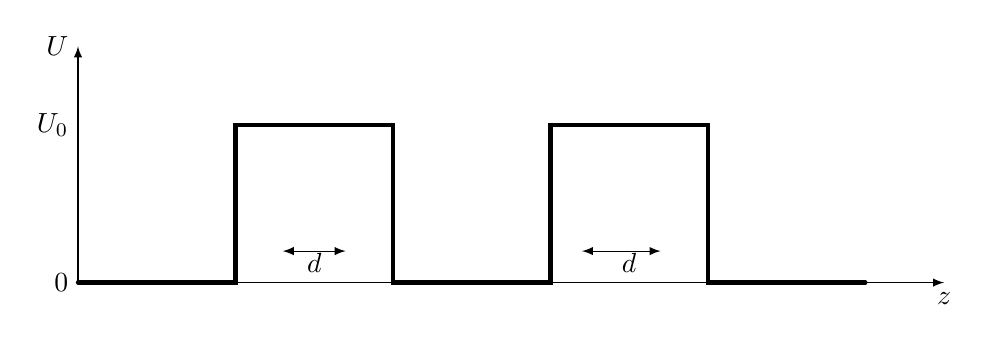
\begin{tikzpicture}[scale=2,cap=round,>=latex]
	\draw [<->] (-2, 1.5) -- (-2, 0) -- (3.5, 0);
	\node [left] at (-2, 1.5) {$U$};
	\node [below] at (3.5, 0) {$z$};
	
	\draw [line width=1.5] (-2, 0) -- (-1, 0) -- 
							(-1, 1) -- (0, 1) -- 
							(0, 0) -- (1, 0) --
							(1, 1) -- (2, 1) --
							(2, 0) -- (3, 0);
							
	\node [left] at (-2, 1) {$U_0$};
	\node [left] at (-2, 0) {$0$};	
	
	\node [above] at (-0.5, 0) {$d$};
	\draw [<->] (-0.7, 0.2) -- (-0.3, 0.2);
		
	\node [above] at (1.5, 0) {$d$};	
	\draw [<->] (1.2, 0.2) -- (1.7, 0.2);
										
\end{tikzpicture}
					\caption{Double quantum barrier system}
				\end{figure}
				
				Calculate the probability of a an electron tunneling through a system of two potential barriers.			
			\paragraph{Minimal transistor size}
				\begin{figure}[!h]
					\centering
					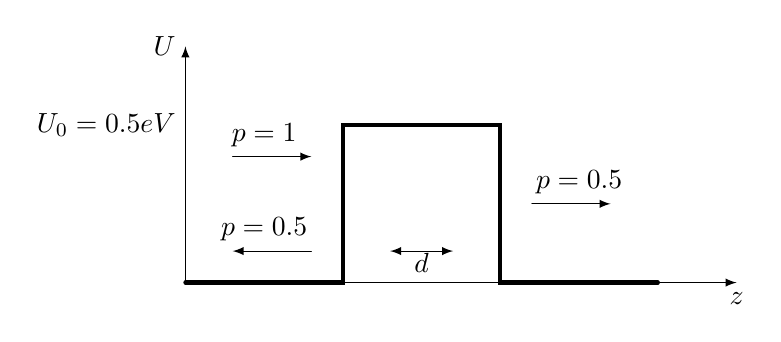
\begin{tikzpicture}[scale=2,cap=round,>=latex]
	\draw [<->] (-2, 1.5) -- (-2, 0) -- (1.5, 0);
	\node [left] at (-2, 1.5) {$U$};
	\node [below] at (1.5, 0) {$z$};
	
	\draw [line width=1.5] (-2, 0) -- (-1, 0) -- (-1, 1) -- (0, 1) -- (0, 0) -- (1, 0);
	
	\node [above] at (-0.5, 0) {$d$};
	\draw [<->] (-0.7, 0.2) -- (-0.3, 0.2);	
	
	\node [left] at (-2, 1) {$U_0 = 0.5\si{eV}$};

	\draw [->] (-1.7, 0.8) -- (-1.2, 0.8);
	\node [above] at (-1.5, 0.8) {$p = 1$};
		
	\draw [<-] (-1.7, 0.2) -- (-1.2, 0.2);
	\node [above] at (-1.5, 0.2) {$p = 0.5$};

	\draw [->] (0.2, 0.5) -- (0.7, 0.5);	
	\node [above] at (0.5, 0.5) {$p = 0.5$};
												
\end{tikzpicture}
					\caption{Model transistor}
				\end{figure}
							
				Calculate the size of a quantum barrier at which an electron's probability of tunneling through is equal to $0.5$.
				\begin{align}
					m_{el} \approx& 0.3 m_0 \\
					m_0 \approx& 10^{-30}\si{kg} \\
					p =& |\Psi|^2
				\end{align}
		\subsubsection{Harmonic oscillator}
			\paragraph{Average values}
				Evaluate the following exrepssions:
				\begin{align}
					\left\langle n|x^2| n\right\rangle = ?\\
					\left\langle n|x| n\right\rangle = ?\\
					\left\langle \Delta x^2 n\right\rangle = ?\\
					\left\langle n|x'| n\right\rangle = ?\\
					\left\langle n|x'^2| n\right\rangle = ? \\																				
				\end{align}				
			